% Chapter 1

\chapter{Introduction} % Main chapter title

\label{Chapter1} % For referencing the chapter elsewhere, use \ref{Chapter1} 

%----------------------------------------------------------------------------------------

% Define some commands to keep the formatting separated from the content 
% \newcommand{\keyword}[1]{\textbf{#1}}
% \newcommand{\tabhead}[1]{\textbf{#1}}
% \newcommand{\code}[1]{\texttt{#1}}
% \newcommand{\file}[1]{\texttt{\bfseries#1}}
% \newcommand{\option}[1]{\texttt{\itshape#1}}

%----------------------------------------------------------------------------------------

% =========================================================== %
%                 Section: General Information                %
% =========================================================== %
\section{General Information}
\label{chap1:sec1:general_information}
This template is for MPhill/Doctor students of University of Hong Kong to prepare their theses. The entire project strictly follows the requirements of \uline{booklet provided by Graduate School of the University of Hong Kong}. The current version of this template is prepared according to the $\boldsymbol{13^\mathrm{th}}$ edition of the booklet entitled ``\href{https://intraweb.hku.hk/reserved_1/gradsch/PreparingandSubmittingYourThesis.pdf}{Preparing and Submitting Your Thesis --- A Guide for MPhil and PhD Students.}'' This edition is updated in \textbf{July 2019}. Considering the university may change the stipulations over time, this template also provides the guidelines to adjust the typeset. The current version of the template has been tested by the author(s) and has been successfully accepted by the Engineering Faculty.
However, \uline{users should also notice that this is not an official template, and we are not responsible for any problems of your thesis preparation and submission caused by using this template.} For anyone who would like to use this template, you have to be responsible for your thesis and your are supposed to carefully read and follow the rules in the latest edition of the university booklet to prepare your thesis. In the rest of the template, we will demonstrate how to use, change, or adjust this template.


% =========================================================== %
%      Section: General Requirements of Graduate School       %
% =========================================================== %
\section{General Requirements of Graduate School}
\label{chap1:sec2:general_requirements_of_graduate_school}
According to the \href{https://intraweb.hku.hk/reserved_1/gradsch/PreparingandSubmittingYourThesis.pdf}{$13^\mathrm{th}$ edition booklet}, ``The Thesis Format'' section, the thesis submitted for examination shall be typewritten or printed on one side or both sides of International size A4 paper, with a margin of not less than 35mm on both right and left-hand edges of each page (as shown in \figref{fig:chap1:thesis_requirements}).
\begin{figure}[!h]
    \centering
    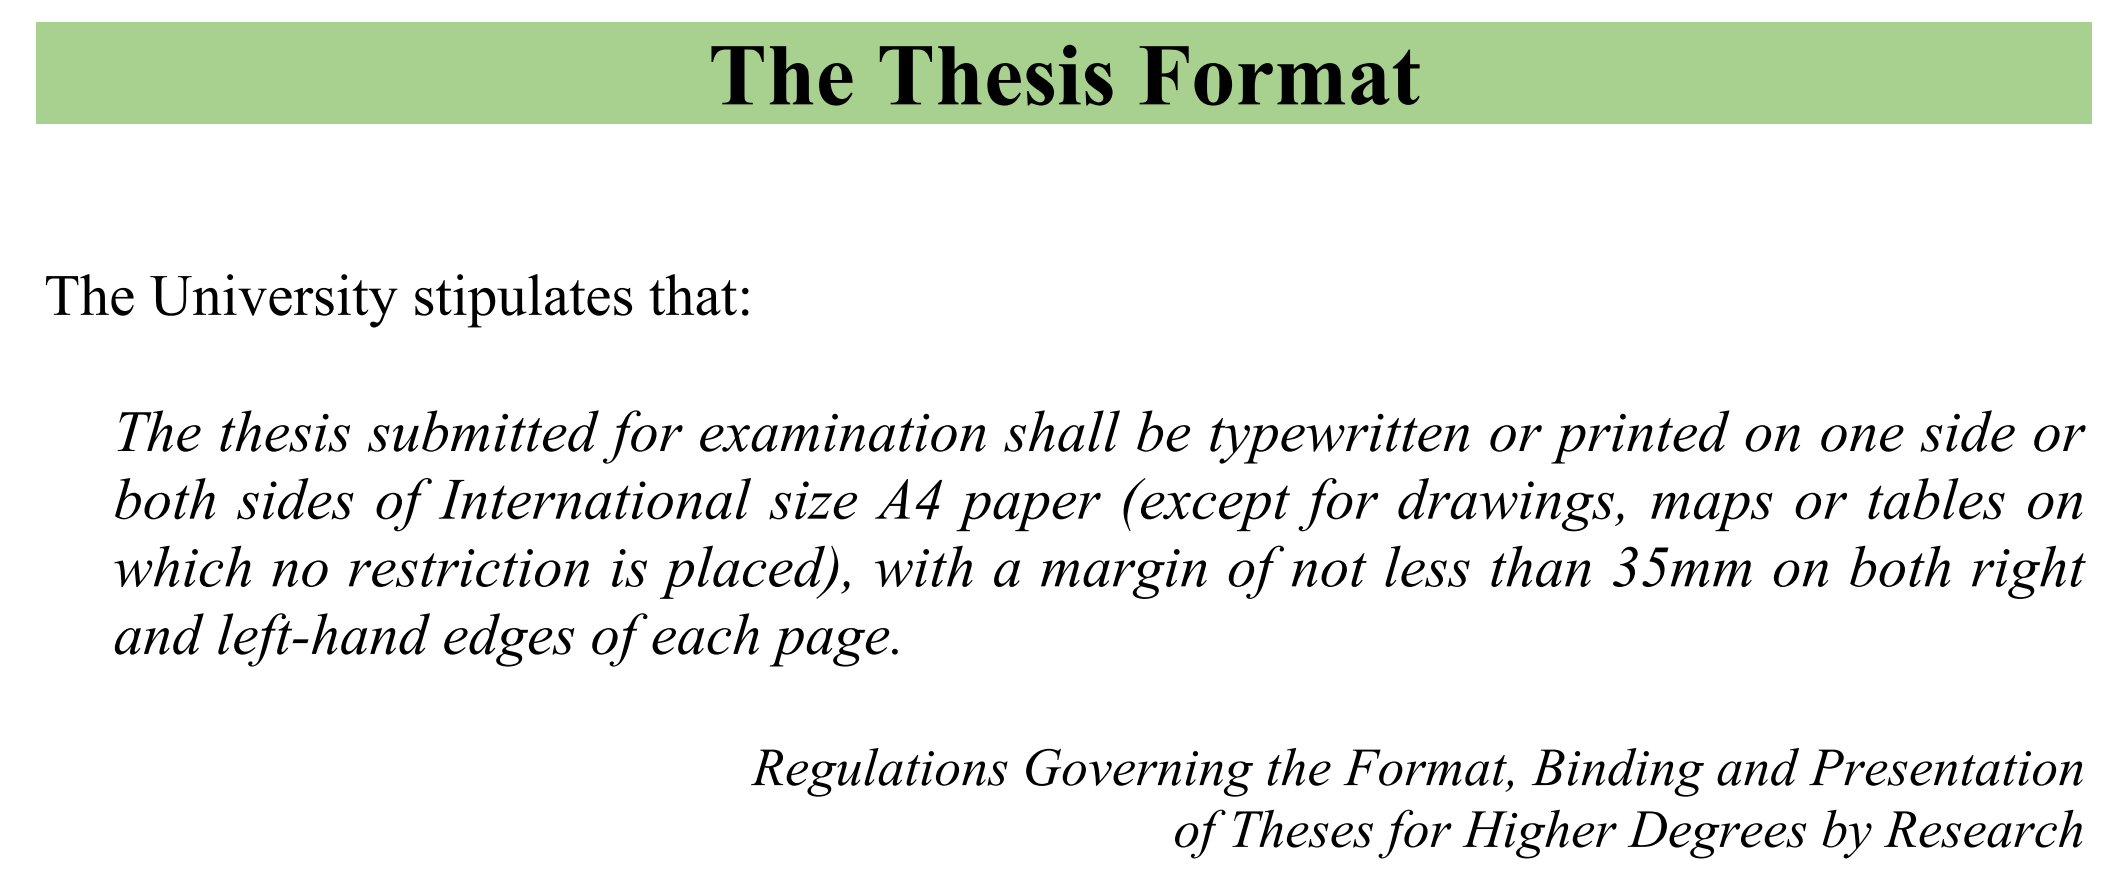
\includegraphics[width=.96\textwidth]{Figures/Chapter1/thesis_requirement.PNG}
    \caption{Requirements of the thesis format in the Graduate School $13^\mathrm{th}$ edition booklet at Page 9.}
    \label{fig:chap1:thesis_requirements}
\end{figure}


% =========================================================== %
%                    Subsection: Page Margin                  %
% =========================================================== %
\subsection{Page Margin}
\label{chap1:sec:2:subsec1:page_margin}
The format of page size and margin is defined in ``main.tex'' file \textbf{Line 63-71}. The page margin of the current version template is \uline{Left: 35mm, Right: 36mm (a4paper).} Users can change the page margin by adjusting the corresponding settings. There is no stipulation for the top and bottom margins, but the booklet recommend that both of them should be 25mm, which is adopted in this template. 


% =========================================================== %
%          Subsection: Font, Alignment, Line Spacing          %
% =========================================================== %
\subsection{Font, Alignment, Line Spacing}
Ordinarily, there is no restrict stipulation for the font family, font size, alignment, and line spacing. All of these are a matter of personal preference. This template uses \textit{10pt} font size, \textit{Fully Justified} alignment style and \textit{One and A Half} line spacing. Users can adjust the settings in \textbf{Line 19-33} of the ``main.tex'' file to change the typeset.


% =========================================================== %
%                      Subsection: Contents                   %
% =========================================================== %
\subsection{Contents}
The contents of this template can be subdivided into three parts --- the front matter, the text and the back matter, which strictly follows the stipulations of the official booklet (Page 17). \tabref{chap1:longtable:checking_list} indicates the what contents are required in the submitted thesis and what contents are optional. The column ``Required'' denotes that 
\begin{center}
\begin{longtable}{|l|c|c|}
\caption{Checking list indicating the contents should be included in the thesis.}\label{chap1:longtable:checking_list}\\
\hline
\textbf{The Front Matter} & Required     &  Include $\checkmark$ \\ \hline \hline
Abstract                  & Yes          & $\checkmark$         \\
Title Page                & Yes          & $\checkmark$         \\
Frontispiece              &              &                      \\
Dedication                &              & $\checkmark$         \\
Epigraph                  &              &                      \\
Declarations              & Yes          & $\checkmark$         \\
Acknowledgements          &              & $\checkmark$         \\
Table of Contents         & Yes          & $\checkmark$         \\
List of Illustrations     &              &                      \\
List of Figures           &              & $\checkmark$         \\
List of Tables            &              & $\checkmark$         \\
List of Algorithm         &              & $\checkmark$         \\
List of Abbreviations     &              & $\checkmark$         \\
List of Symbols           &              & $\checkmark$         \\
Others                    &              &                      \\ \hline \hline
\textbf{The Text}         & Yes          & $\checkmark$         \\ \hline \hline
\textbf{The Reference or Back Matter} &    ---    &   ---       \\ \hline \hline
Glossary                  &              &                      \\
Appendices                &              &                      \\
Notes                     &              &                      \\
Bibliography or Reference List & Yes          &  $\checkmark$   \\
Index                     &              &                      \\
\hline
\end{longtable}
\end{center}
This template support most of the contents listed in the figure, including the ``Abstract'', ``Title Page'', ``Declarations'', ``Acknowledgements'', ``List of Publications'', ``Contents'', ``List of Figures'', ``List of Tables'', ``List of Algorithms'', ``List of Abbreviations'', ``List of Symbols'', ``Main Text'', ``Appendices'', and ``Bibliography''. Each part is defined in an independent tex file and the ``main.tex'' file combines all the different parts to form the entire thesis. Therefore, users can easily make the changes by adjusting the corresponding document files.

In addition to the stipulations of the booklet, this template also provides a beautiful \textbf{cover page}, which is the first two pages of this project. \uline{The cover page is \textbf{not required} by the Graduate School and you'd better remove the cover page when bounding your thesis for submission.}








